\section{Fuzzing de Radare2}

%%%%%%%%%%%%%%%%%%%%%%%%%%%%%%%%%%%%%%%%%%%%%%%%%%%%%%%%%%%%%%%%%%%%%%%%%
% Présentation de Radare2
%%%%%%%%%%%%%%%%%%%%%%%%%%%%%%%%%%%%%%%%%%%%%%%%%%%%%%%%%%%%%%%%%%%%%%%%%
\begin{frame}{Fuzzing de Radare2}{Pourquoi Radare2 ?}
  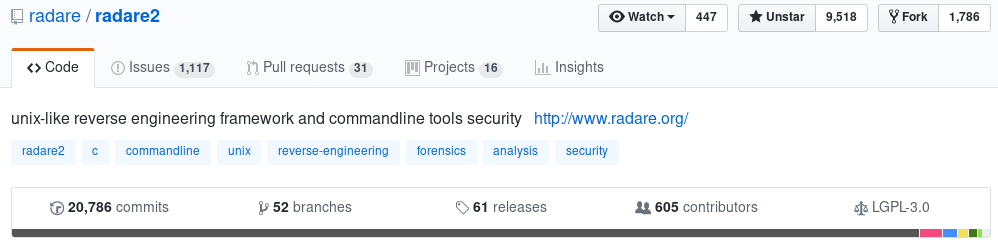
\includegraphics[width=\linewidth]{../medias/radare2-github.png}
  \begin{exampleblock}{Radare2 en quelques mots}
    \begin{itemize}
    \item{outil de reverse-engineering opensource (GPLv3)}
    \item{40+ architectures (x86, ARM, MIPS, SPARC...)}
    \item{30+ formats (ELF, PE, DEX...)}
    \item{écrit en C (bugs de corruption mémoire)}
    \item{20000+ commits, 600+ contributeurs, 900K+ LoC}
    \end{itemize}
  \end{exampleblock}
\end{frame}

%%%%%%%%%%%%%%%%%%%%%%%%%%%%%%%%%%%%%%%%%%%%%%%%%%%%%%%%%%%%%%%%%%%%%%%%%
% Présentation de la méthodologie
%%%%%%%%%%%%%%%%%%%%%%%%%%%%%%%%%%%%%%%%%%%%%%%%%%%%%%%%%%%%%%%%%%%%%%%%%
\begin{frame}[fragile]{Fuzzing de Radare2}{Méthodologie}
  \begin{block}{Méthodologie}
    \begin{itemize}
    \item{installation de AFL}
    \item{instrumentation de Radare2 grâce à \lstinline{afl-gcc}}
    \item{établir une base d'entrées initiales pour alimenter le fuzzer}
    \item{fuzzing de Radare2 avec \lstinline{afl-fuzz}}
    \item{analyse des résultats avec Address Sanitizer}
    \end{itemize}
  \end{block}

  \pause

  \begin{exampleblock}{Récupération des sources}
    \begin{itemize}
    \item{\url{http://lcamtuf.coredump.cx/afl/releases/afl-latest.tgz}}
    \item{\url{https://github.com/radare/radare2}}
    \end{itemize}
  \end{exampleblock}

  \pause
  \vfill

  \begin{exampleblock}{Instrumentation de radare2}
    \begin{itemize}
    \item \lstinline{CC=afl-gcc ./sys/user.sh --install-path ../radare2-install}
    \end{itemize}
  \end{exampleblock}

\end{frame}


%%%%%%%%%%%%%%%%%%%%%%%%%%%%%%%%%%%%%%%%%%%%%%%%%%%%%%%%%%%%%%%%%%%%%%%%%
% Entrées de Radare2
%%%%%%%%%%%%%%%%%%%%%%%%%%%%%%%%%%%%%%%%%%%%%%%%%%%%%%%%%%%%%%%%%%%%%%%%%
\begin{frame}[fragile]{Fuzzing de Radare2}{Génération des entrées}
  \begin{center}
    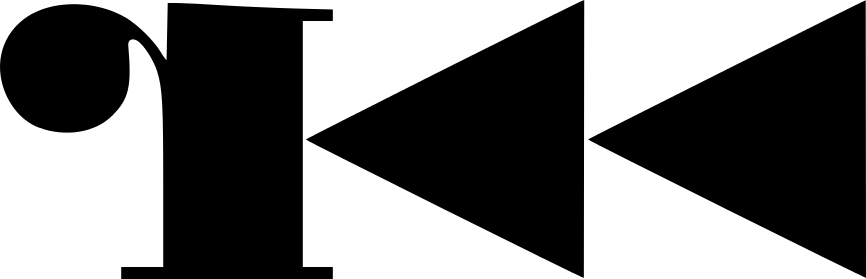
\includegraphics[width=0.25\textwidth, clip=true]{../medias/radare2-logo.png}
  \end{center}

  \begin{columns}[T]
    \begin{column}{0.44\linewidth}

      \begin{block}{Analyseur de fichiers}
        \begin{itemize}
        \item{\path{binary-samples/}}
        \item{\path{radare2-regressions/}}
        \item{sélection de petits binaires}
        \item{$\ne$ architectures/formats}
        \end{itemize}

        \vspace{1.75ex}
      \end{block}
    \end{column}

    \begin{column}{0.44\linewidth}
      \begin{block}{Interpréteur de commandes}
        \begin{itemize}
        \item{1 caractère = 1 action}
        \item{\lstinline{px} = ``Print hexdump''}
        \item{\lstinline{pxj} = ``Print hexdump in JSON''}
        \item{élaboration de scripts}
        \end{itemize}
      \end{block}
    \end{column}
  \end{columns}
  \pause
  \vfill
  \begin{exampleblock}{Autres outils}
    \begin{itemize}
    \item{\lstinline{rax2}, \lstinline{rabin2}, \lstinline{rafind2}, \lstinline{rasm2}, \lstinline{radiff2}, ...}
    \end{itemize}
  \end{exampleblock}
\end{frame}

%%%%%%%%%%%%%%%%%%%%%%%%%%%%%%%%%%%%%%%%%%%%%%%%%%%%%%%%%%%%%%%%%%%%%%%%%
% afl-fuzz en pratique
%%%%%%%%%%%%%%%%%%%%%%%%%%%%%%%%%%%%%%%%%%%%%%%%%%%%%%%%%%%%%%%%%%%%%%%%%
\begin{frame}{Fuzzing de Radare2}{afl-fuzz}
  \begin{figure}
    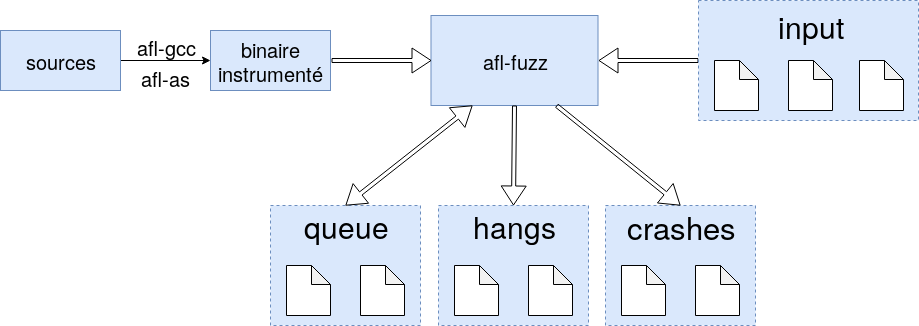
\includegraphics[width=0.98\linewidth]{../medias/afl-overview.png}
  \end{figure}

  \pause

  \begin{exampleblock}{afl-fuzz}
    \begin{itemize}
    \item{serveurs de calculs du CREMI : 48 CPU + 128 Go de RAM}
    \item{10 instances d'\lstinline{afl-fuzz}}
    \item{en tout, environ 1 semaine de fuzzing}
    \end{itemize}
  \end{exampleblock}

\end{frame}

\begin{frame}{Fuzzing de Radare2}{afl-fuzz}
  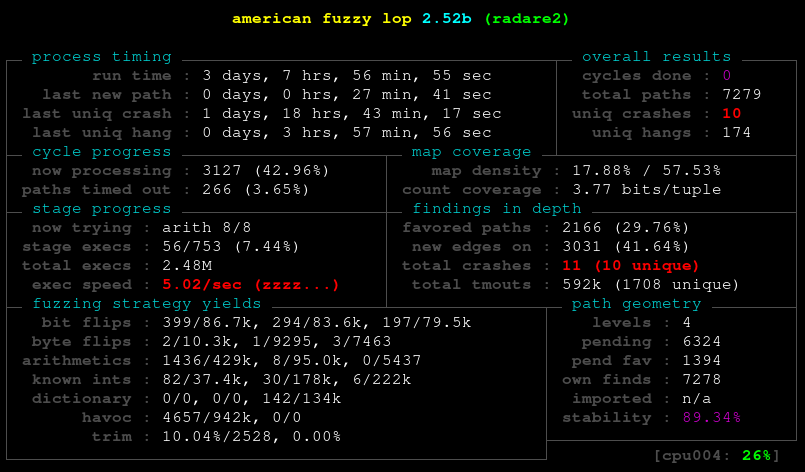
\includegraphics[width=\linewidth]{../medias/afl-fuzz.png}
\end{frame}

%%%%%%%%%%%%%%%%%%%%%%%%%%%%%%%%%%%%%%%%%%%%%%%%%%%%%%%%%%%%%%%%%%%%%%%%%
% Résultats
%%%%%%%%%%%%%%%%%%%%%%%%%%%%%%%%%%%%%%%%%%%%%%%%%%%%%%%%%%%%%%%%%%%%%%%%%
\begin{frame}{Fuzzing de Radare2}{Résultats}
  \begin{exampleblock}{Address Sanitizer (ASan)}
    \begin{itemize}
    \item{développé par Google}
    \item{instrumentation basée sur LLVM}
    \item{détecte certaines corruptions mémoires (overflows, UAF...)}
    \end{itemize}
  \end{exampleblock}

  \pause

  \begin{block}{Résultats}
    \begin{itemize}
    \item{10 bugs remontés et corrigés par Radare2}
    \item{3 read out-of-bounds}
    \item{2 double-free}
    \item{2 bad-pointer-dereference}
    \item{1 use-after-free}
    \item{1 stack-based-overflow}
    \item{1 integer-overflow}
    \end{itemize}
  \end{block}
\end{frame}

\begin{frame}[fragile]{Fuzzing de Radare2}{Exemple de bug trouvé}
  \begin{lstlisting}[language=C]
  case ' ': ;// "db"
    for ( ; i < sl; i += 1 + (watch ? 1 : 0)) {
      if (*DB_ARG(i) == '-') {
        /* ... */
      } else {
        /* ... */
        if (!strcmp (DB_ARG (i + 1), "r")) {
          rw = R_BP_PROT_READ;
        } else if (!strcmp (DB_ARG (i + 1), "w")) {
          /* ... */
        } else {
          r_core_cmd_help (core, help_msg_dbw);
          free (str);
          break;
        }
      }
    }
    free (str);
    break;

  case 'i':
    /* ... */
  \end{lstlisting}
\end{frame}
